\documentclass[12pt]{article}
\usepackage[utf8]{inputenc}
\usepackage{fullpage}
\usepackage{graphicx}
\usepackage{hyperref}

\begin{document}

\section*{Introduction}

High-speed data throughput is a requirement for most high energy physics software. Whether improving old software or developing new software, we must keep an eye on this aspect of its performance.

The metrics described in this section were measured as part of the development process for two new software products: root4j\footnote{\url{https://github.com/diana-hep/root4j}}, which provides access to ROOT files in Java (and therefore Apache Spark), and Femtocode\footnote{\url{https://github.com/diana-hep/femtocode}}, which is a query system, intended to produce plots from large (petabyte) datasets in real time.

Throughput bottlenecks can appear in three places. The first is loading into memory, which includes reading from physical disks and the network, deserialization, and decompression. The second is loading from memory into the processing unit, which is often much faster than the first and doesn't involve any transformations. The third is the computation itself. All three are relevant because caches may be employed to hide the effect of a slow load-into-memory or a slow load-from-memory.

For instance, root4j is called by spark-root\footnote{\url{https://github.com/diana-hep/spark-root}} to load data from ROOT files into Spark as a {\tt DataFrame}. After the first request (and until subsequent loads cause it to spill to disk), Spark caches the {\tt DataFrame}, distributing its contents across the random access memory of a whole cluster. Similarly, Femtocode is designed with the expectation that physicist users want to re-plot the same data several times in a row, tweaking aspects of the plot, so it also has a distributed, in-memory cache. In the first request, the disk or network bottleneck is relevant; afterward, the memory-to-processor bandwidth is relevant. The calculation itself may or may not overwhelm both of these, depending on what is being calculated. Simple histogram filling (the most common use-case for both Spark and Femtocode) requires much less processing time than load time.

We will therefore focus on the first two bottlenecks only: load-to-memory and memory-to-processor. Furthermore, each of these depend strongly on the hardware. Our software may be used on any hardware, so each of our metrics is a {\it comparison} of one software solution to another, both on the same hardware. These numbers should therefore be understood as relative, except where the specific hardware is described.

Code for all of these tests can be found in the {\tt diana-hep/femtocode-metrics} GitHub repository\footnote{\url{https://github.com/diana-hep/femtocode-metrics}}.

\section*{ROOT file reading: Java vs optimized C++}

The root4j library is a pure-Java implementation of ROOT file reading. This has technical advantages over alternatives that would call the standard C++ implementation of ROOT (JNI, UNIX pipes, or sockets): root4j is easy to install as a JAR from Maven Central and is free of several classes of bugs, including segmentation faults and failures in interprocess communication. It does, however, have the potential to be slower than the C++ implementation, since Java is a virtual machine with garbage collection.

Early in the development process, the read performance of root4j and C++ ROOT was compared to get a sense of this cost. Track $\chi^2$ values for all tracks (hundreds per event) were read from a CMS public dataset (AOD). This study focuses on a single attribute of a variable-length collection of objects within the event, so it relies heavily on the fact that these objects are laid out in a columnar fashion in the ROOT files.

Figure~\ref{root4j_reading_tracks} shows the reading rate as nanoseconds per track (left axis) and, equivalently, as megabytes per second for the {\it decompressed} data (right axis), measured every 100,000 tracks. Measuring this rate as a function of time is important because Java does HotSpot optimization at the beginning of the run, sacrificing start-up latency for long-term throughput.

\begin{figure}
\begin{center}
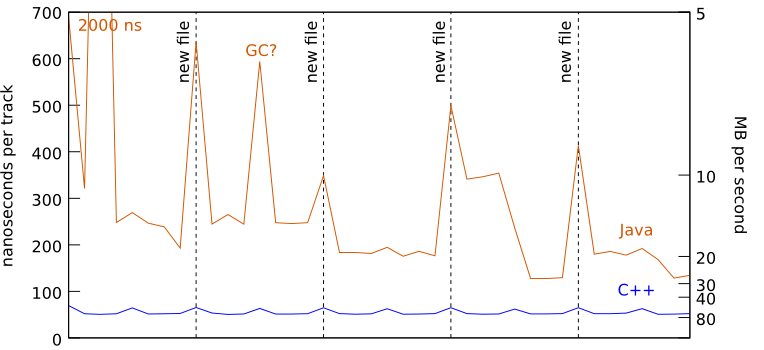
\includegraphics[width=0.8\linewidth]{root4j_reading_tracks.png}
\end{center}

\caption{\label{root4j_reading_tracks} Rate of reading track $\chi^2$ in root4j and C++ ROOT as a function of time. (Samples on the horizontal axis are every 100,000 tracks and ``MB'' refers to {\it decompressed} data.)}
\end{figure}

These files were also pre-read before measuring any data, so that they would be in Linux's memory cache, effectively removing the physical bottleneck of disk access and ensuring that neither software product is unfairly discounted because of this large bottleneck.

Both C++ and Java readers are deserializing and decompressing (zip) the same bytes. The C++ ROOT version is 6.08/04 (pre-built binary for Ubuntu Linux). The root4j version is 0.1-pre2; spark-root and Spark were {\it not} involved in this test (which would complicate matters, due to caching). Both have been executed in a single process, single thread.

In the plot, we see that standard C++ ROOT is consistently faster than root4j. We also see that, unlike C++, root4j starts slow and accelerates. We see the HotSpot optimization phase as a spike (temporary slow-down) at the beginning of reading, a spike when opening each file, and a single spike in the middle of one file read. Spikes like these appear at different times in different runs, so they are likely garbage collector pauses.

However, the asymptotic speed of root4j, which is all that matters for large files and large datasets, is about four times slower than C++. Depending on the user's intended purpose, this cost may be worthwhile, since it opens direct access to all the ``big data'' and machine learning tools that have been developed for the Java platform.

More recent performance benchmarks are in development, using Spark's built-in performance counters\footnote{\url{https://github.com/diana-hep/spark-root/blob/master/md/PerformanceBenchmarksPublicDS.md}}.

\section*{ROOT file reading: CMSSW vs optimized C++}

This second test of ROOT file reading was motivated by Femtocode, which takes advantage of ROOT's columnar data representation in files to performs calculations on data in this same form in memory, without reconstructing objects. This is in contrast to a traditional framework for analyzing physics data, such as CMSSW.

CMSSW uses ROOT to build instances of C++ classes, and physicist users write C++ code to interact with those instances. Since arbitrary-length collections of record structures ({\tt std::vector<SomeClass>}) are common, these objects may not be contiguous in memory. Since the user code could access any attribute of these classes, all columns associated with the whole class must be loaded, even if the user actually accesses only one or two.

Femtocode, on the other hand, is a high level language that gets JIT-compiled to machine code. Part of this compilation process determines which attributes are needed and only loads those. Furthermore, the code is compiled in a way that can act on contiguous arrays of data loaded directly from the ROOT file, so construction of objects is not necessary.




\section*{Memory bandwidth: conventional vs GPU vs KNL}

\end{document}
